% !TEX root =  master.tex
\chapter{Evolutionäre und genetische Algorithmen zur Bewältigung komplexer Aufgaben}

In diesem Paper geht es um die Thematik von Trading Bots im Bereich der evolutionären und genetischen Algorithmen. 
Mit dem Handel an Börsen und vor allem dem sehr schnellen Kauf und Verkauf der dort gehandelten Papiere und Währungen ist die Nachfrage an digitalen Unterstützungen gewachsen. \cite{admirals_2018} Um noch bessere Ergebnisse durch intelligentes Kaufen und Verkaufen von Wahren zu schaffen, werden auch hierbei Rechenmaschinen zur Unterstützung herangezogen. Die Robotik, welche hier zum Einsatz kommt wird Trading Bot genannt. \cite{scheuschner_2021} Vor allem mit dem großen Boom digitaler Währungen, wie zum Beispiel Bitcoin, ist die Nachfrage an eben solchen Trading Bots enorm gestiegen. \cite{scheuschner_2021} Denn so kann, ohne permanente Konzentration auf das Marktgeschehen, am Markt partizipiert werden. Grund dafür ist, dass die Trading Bots von der Analyse des Marktes bis zum Kauf und Verkauf von Währungen oder Aktien autark agieren.

In dieser wissenschaftlichen Ausarbeitung werden zwei unterschiedliche Verfahren von Trading Bots miteinander Verglichen und gegenübergestellt. Zum einen wird ein Regelbasierter \enquote{Buy Low Sell High} Algorithmus implementiert, welcher später als Basis zum Vergleich dient. Des Weiteren wird ein Reinforcement Learning Ansatz erstellt, welches anhand von Q-Learning ein Modell lernt, das dann wiederum den eigentlichen Handel anhand seiner Einschätzung der Situation durchführt. Beide Modelle wurden zum Vergleich implementiert. Dabei ist darauf hinzuweisen, dass die Implementierungen nicht vollständig in Eigenleistung erstellt wurden, sondern sich beim Q-Learning Modell auf eine Implementierung des Blogs Analytics Vidhya \cite{analyticsvidhya_2021} und beim Regelbasierten Verfahren auf die Umsetzung von Willems \cite{willems_2019} angelehnt wurde.

Im Folgenden werden die Ansätze beider Modelle kurz erläutert. Nähere Informationen zur detaillierten Implementierung finden sich im Quelltext der jeweiligen Umsetzung, welche jeweils umfänglich dokumentiert sind.
Die Daten und somit auch deren Import, also das Laden der Daten in die Funktion, ist für beide Modelle gleich. Wichtig ist dies, damit die Vergleichbarkeit beider Algorithmen gegeben ist. Mit dem Paket \enquote{pandas-datareader} ist es möglich, Daten aus Quellen wie z.B. Google, Weltbank oder Yahoo-Finance einzulesen. \cite{willems_2019} Für die hier vorliegende Implementierung werden Daten des Apple Aktienkurses geladen und in die dafür bereitgestellten Pandas Dataframes gelegt. Das daraus resultierende Objekt ist vom Typ \enquote{aapl} und Förmlich eine 2-dimensionale, beschriftete Datenstruktur mit Spalten, potenziell unterschiedlicher Typen. \cite{willems_2019} Die erste Spalte wird verwendet, um die Anzahl der Aktien zu registrieren, die an einem einzigen Tag gehandelt wurden. \cite{willems_2019} Letzterer ist andererseits der bereinigte Schlusskurs: Es ist der Schlusskurs des Tages, der leicht angepasst wurde, um alle Aktionen zu berücksichtigen, die zu einem beliebigen Zeitpunkt vor der Eröffnung des nächsten Tages stattgefunden haben.  \cite{willems_2019} Diese Spalte kann zur Untersuchung respektive detaillierten Analyse historischer Renditen herangezogen werden. \cite{willems_2019} 

Der Regelbasierte Algorithmus ist eine einfache Momentum-Strategie und Teil des quantitativen Handels, dem Moving Average Crossover. \cite{willems_2019} Die Strategie der Implementierung ist indes simpel. Es werden zwei separate \ac{SMA} einer Zeitreihe mit unterschiedlichen Lookback-Perioden (in diesem Fall 40 und 100 Tage) erstellt. \cite{willems_2019} Wenn der kurze Abschnitt den längeren überbietet, wird gekauft, wenn der längere den kurzen Abschnitt überbietet, wird verkauft. \cite{willems_2019} Das schrittweise Vorgehen dabei lautet: \cite{willems_2019}
\begin{itemize}
	\item Zwei unterschiedliche Lookback-Perioden setzen, ein kurzes und langes Fenster. Jeder Variable sollte eine Ganzzahl zugewiesen werden, das lange Fenster hat dabei den höheren Wert gegenüber dem kleinen.
	
	\item Im zweiten Schritt wird ein Signal Datensatz initiiert. Dafür wird die geladene aapl-Datei kopiert, damit die Berechnung des Kauf- oder Verkaufssignals umgesetzt werden kann.
	
	\item Im erzeugten Datensatz wird eine Spalte mit dem Namen \enquote{signal} mit dem Wert \enquote{0.0} für jede Zeile initialisiert.

	\item Mit dem Aufruf der Funktion \enquote{rolling()} wird die Rolling-Window-Berechnung gestartet. Das heißt, die vorher definierten kurzen und langen \ac{SMA} über die jeweiligen Zeitfenster  werden erstellt. Innerhalb der Funktion wird das Fenster und die \enquote{min\_period} angegeben und legt damit das Center-Argument fest. In der Praxis führt dies zu der besagten \enquote{rollenden}-Funktion.
	
	\item Nachdem die Mittelwerte der kurzen und langen Fenster berechnet wurden, wird ein Signal erzeugt, wenn der kurze \ac{SMA} den langen \ac{SMA} schneidet, jedoch nur für den Zeitraum, der größer als das kürzeste \ac{SMA} ist. Ist diese Bedingung wahr, wird der initialisierte Wert 0.0 in der Signalspalte mit 1.0 überschrieben. Im anderen Fall, also wenn die Bedingung falsch ist, wird der ursprüngliche Wert von 0.0 beibehalten und es wird kein Signal generiert. 

	\item Am Ende wird die Differenz der Signale genommen, um tatsächliche Handelsaufträge zu generieren. Mit anderen Worten, in dieser Spalte des Signal-Datensatzes kann zwischen Long- und Short-Positionen unterschieden werden, unabhängig davon, ob Aktien gekauft oder verkauft wurden.
\end{itemize}


Beim Reinforcement Learning handelt es sich um eine Art des maschinellen Lernens, bei der es Umgebungen und Agenten gibt. \cite{analyticsvidhya_2021} Das Ziel dieser Agenten ist es, anhand von getätigten Schritten zu evaluieren, ob dieser positiv oder negativ war und entsprechen eine Belohnung auszuschreiben. Für den hier vorliegenden Anwendungsfall wird ein Q-Learning Algorithmus angewandt, welcher zum modellfreien Reinforcement Learning zählt. \cite{analyticsvidhya_2021} Es teilt dem Agenten mit, welche Maßnahmen den Umständen entsprechend zu ergreifen sind und handelt sich dabei um eine wertbasierte Methode, die verwendet wird, um einem Agenten Informationen für die bevorstehende Aktion bereitzustellen. \cite{analyticsvidhya_2021} Das \enquote{Q} steht hierbei für Qualität und bezieht sich auf die Aktionsqualität, welche darauf abzielt, wie nützlich diese Belohnung in Übereinstimmung mit der ergriffenen Aktion ist. \cite{analyticsvidhya_2021} Die im Quelltext definierte Funktion liefert uns dabei die maximale Belohnung am Ende der N-ten Anzahl von Trainingszyklen. Mögliche Aktionen des Agenten sind dabei:
\begin{itemize}
	\item Kaufen
	\item Verkaufen
	\item Halten
\end{itemize}

Q-Learning bewertet dabei jede einzelne Aktion, wobei die mit dem maximalen Wert weiter ausgewählt wird. \cite{analyticsvidhya_2021} Da die Belohnungsfunktion und Übergangswahrscheinlichkeit beim Börsenhandel nicht bekannt sind, ist das modellfreie Q-Learning von großer bedeutung. Zuerst wird der Agent Definiert. Danach wird die erste Funktion der Agent-Klasse, welche die Zustandsgröße, Fenstergröße, Stapelgröße, Deque (verwendeter Speicher) und Inventar als Liste definiert. \cite{analyticsvidhya_2021} Im weiteren Verlauf wird auch ein Gradient Descent Optimizer benutzt um das Modell zu verbessern. Der Agent hat für Kauf- und Verkaufsoptionen definierte Funktionen, die Funktion \enquote{get\_state} verwendet das neuronale Netz, um den nächsten Zustand des neuronalen Netzes zu erzeugen. \cite{analyticsvidhya_2021} Die Belohnungen werden anschließend berechnet, indem der durch die Ausführung der Call-Option generierte Wert addiert oder subtrahiert wird. \cite{analyticsvidhya_2021} Die im nächsten Zustand ausgeführte Aktion wird durch die im vorherigen beeinflusst. \cite{analyticsvidhya_2021} 1 bezieht sich auf einen Buy-Call, während sich 2 auf einen Sell-Call bezieht. \cite{analyticsvidhya_2021} In jeder Iteration wird der Zustand bestimmt, auf dessen Grundlage eine Aktion ausgeführt wird, die Aktien entweder kauft oder verkauft. \cite{analyticsvidhya_2021} Die Gesamtprämien werden in der Variable Gesamtgewinn gespeichert. \cite{analyticsvidhya_2021}

Nach der vollständigen Implementierung und einigen Tests wurde der Q-Learning Agent gelernt und parallel zum Baseline Modell ausgeführt. Dabei sind unterschiedliche Ergebnisse entstanden, die im folgenden erläutert werden. Zuerst wird auf die Unterschiede eingegangen, die beim Q-Learning mit unterschiedlicher Anzahl an Lern-Epochen entstanden sind. 

Nach dem Lernen von 10 Epochen agiert das Model stabil und erreicht einen Investitionswert von 0.013\% was eine erste gute Leistung ist, da kein Verlust erwirtschaftet wurde.
\begin{figure}[H]
	\centering
	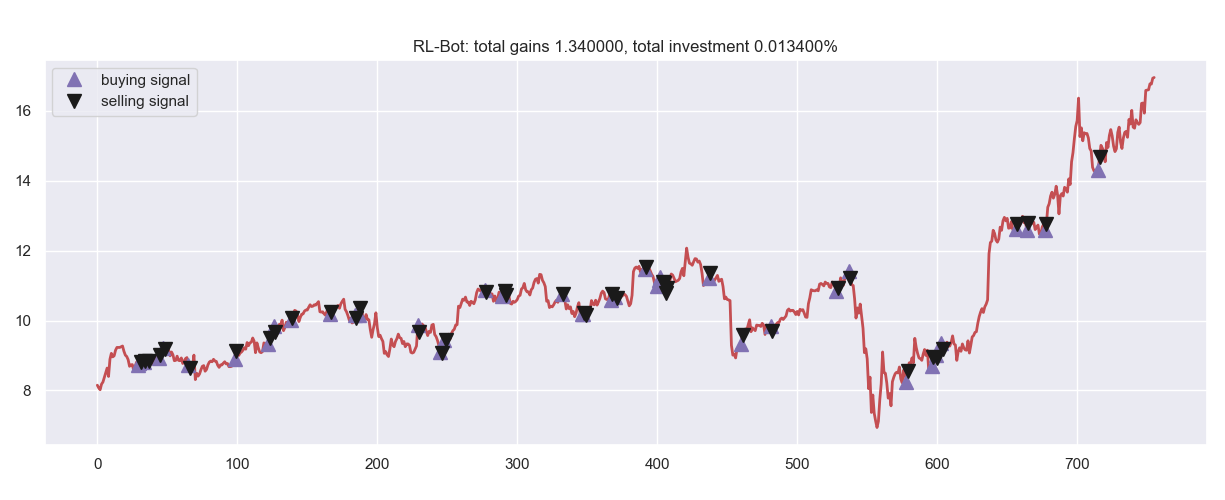
\includegraphics[scale=0.5]{../Topic3-TradingBot/plots/10iter-RL-bot.png} \caption{Q-Learning Agent mit 10 Lern-Iterationen}
\end{figure}

Nach 20 Lernepochen kann eine deutliche Verbesserung festgestellt werden, da der Agent bereits viel mehr Aktionen durchführt. Dies ist auch am Investitionswert von bereits 0.059\% zu erkennen.

\begin{figure}[H]
	\centering
	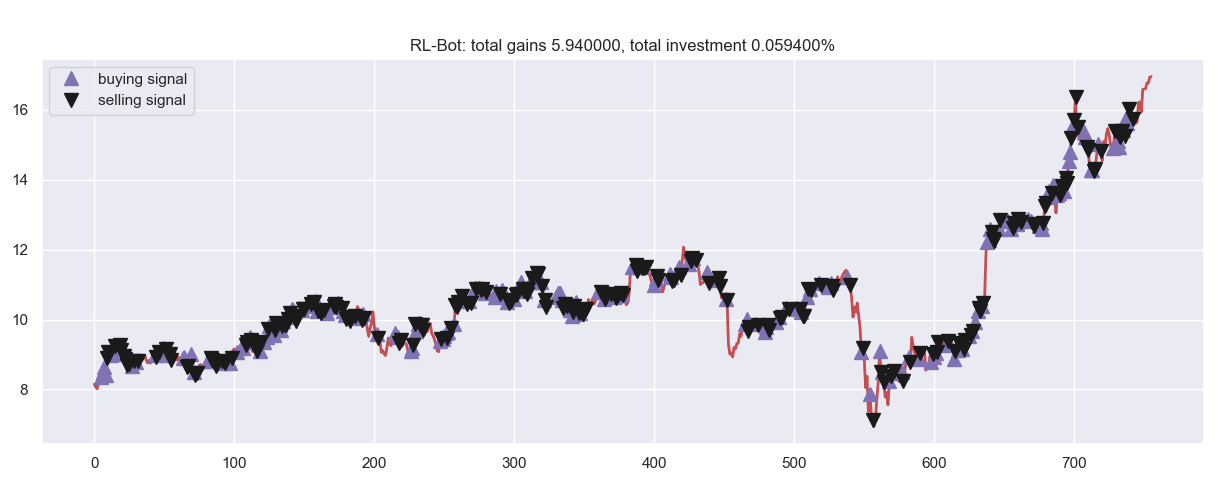
\includegraphics[scale=0.5]{../Topic3-TradingBot/plots/50iter-RL-bot.png} \caption{Q-Learning Agent mit 50 Lern-Iterationen}
\end{figure}

Mit 100 und den darauffolgenden 200 Iterationen beim lernen scheint der Agent eher schlechtere Ergebnisse zu erzielen. Beim ersteren werden nur sehr wenig Aktionen getätigt und beim anderen übermäßig viele. Der Agent mit 100 Lernepochen verzeichnet mit einem Investitionswert von 0.007\% noch ein positives Ergebnis, wobei der zweite Agent sogar ein negatives Investment von ganzen 4.5\% erreicht. Hieraus zeichnet sich eine klare, mit der Anzahl Epochen, steigende Fehlerquote ab. 

\begin{figure}[H]
	\centering
	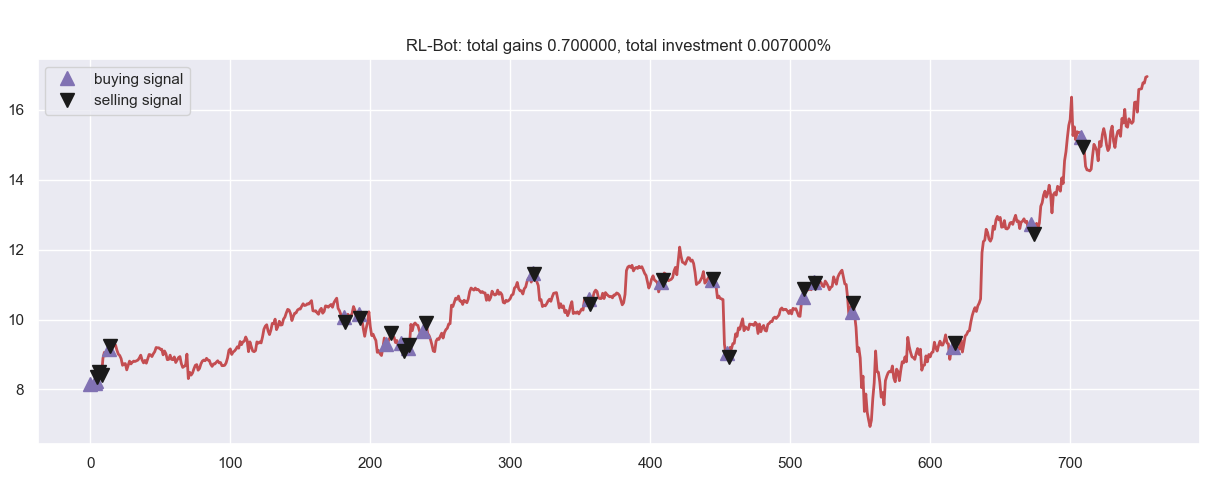
\includegraphics[scale=0.5]{../Topic3-TradingBot/plots/100iter-RL-bot.png} \caption{Q-Learning Agent mit 100 Lern-Iterationen}
\end{figure}

\begin{figure}[H]
	\centering
	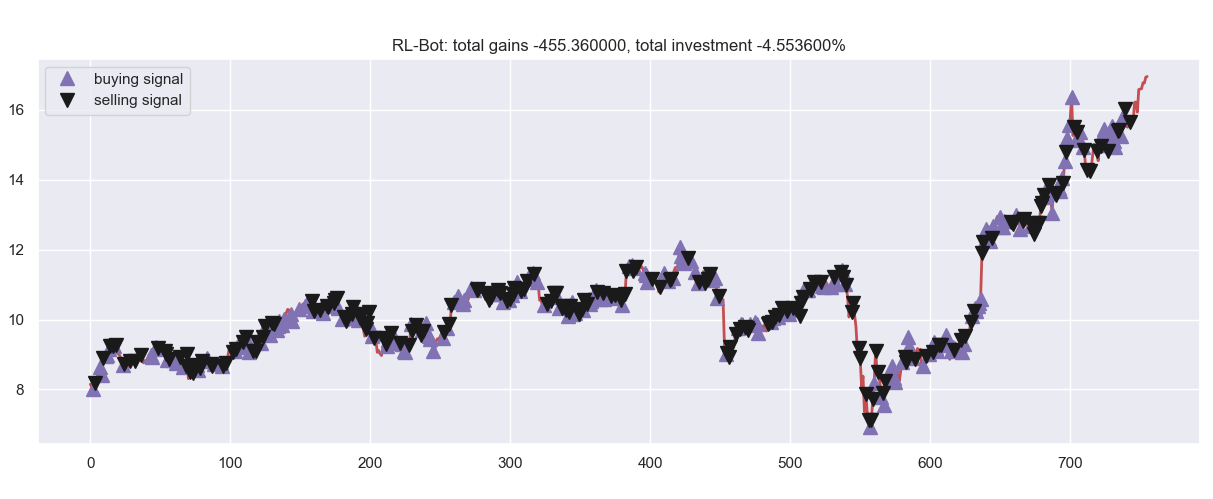
\includegraphics[scale=0.5]{../Topic3-TradingBot/plots/200iter-RL-bot.png} \caption{Q-Learning Agent mit 200 Lern-Iterationen}
\end{figure}

Der Basisansatz verzeichnet ebenfalls gute Ergebnisse Analog dem Q-Learning Agenten. Hier geht klar hervor, dass eher weniger Aktionen durchgeführt werden, da eine Aktion erst nach Analyse der sich verschiebenden Zeitfenster getätigt werden kann. Die Ergebnisse des Modells sind für die geringe Komplexität sehr gut.

\begin{figure}[H]
	\centering
	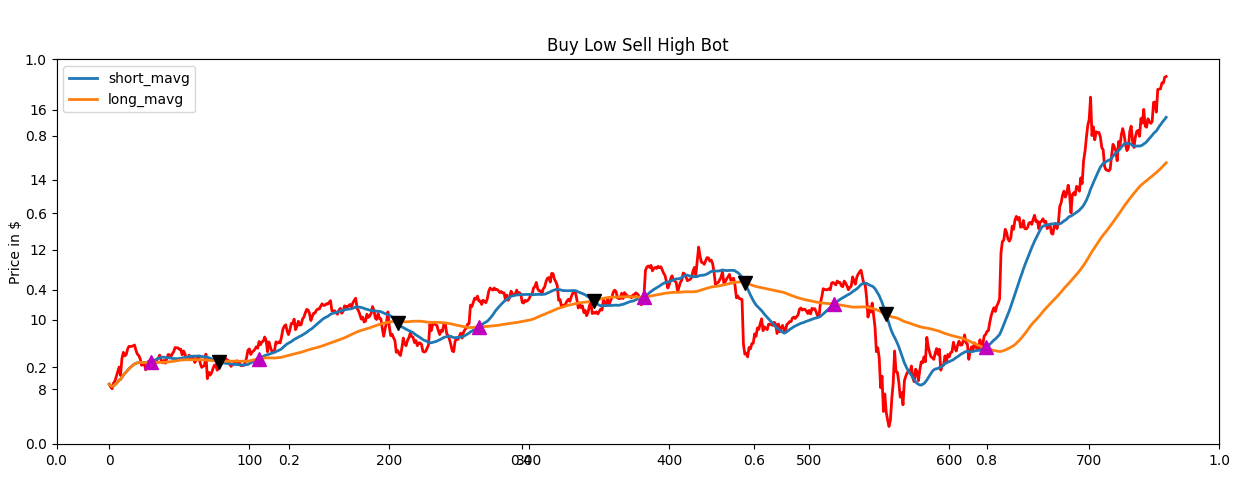
\includegraphics[scale=0.5]{../Topic3-TradingBot/plots/BLSH-bot.png} \caption{Buy Low Sell High Heuristik}
\end{figure}
